\documentclass[a4paper]{article}
% Shared preamble for the English probability and statistics documents.
% Based on the original course preamble. Compile with pdfLaTeX.
\usepackage[top=1.5cm,bottom=2cm,left=2cm,right=2cm]{geometry}
\usepackage[T1]{fontenc}
\usepackage{lmodern}
\usepackage[utf8]{inputenc}
\usepackage[english]{babel}

\usepackage{amsmath}
\usepackage{amssymb}
\usepackage{amsthm}
\usepackage{mathrsfs}
\usepackage{mathtools}
\usepackage{etoolbox}
\usepackage{tikz}
\usetikzlibrary{shapes.multipart,arrows.meta}
\usepackage{xcolor}
\usepackage{enumerate}
\usepackage[shortlabels]{enumitem}
\usepackage{hyperref}
\usepackage{version}
\usepackage{bbold}
\usepackage{fontawesome5}
\usepackage{fancyhdr}
\lfoot{}
\usepackage{natbib}
\usepackage{graphicx}
\usepackage{pdfpages}
\usepackage{authblk}
    
\usepackage{blindtext}
\usepackage{multicol}
\usepackage{collcell}
\usepackage{wrapfig}
\usepackage{blkarray}
\usepackage{cancel}
\usepackage{appendix}
\usepackage{float}
\makeatletter
\input{tex/assets/slashbox.sty}
\makeatother
\hypersetup{unicode,colorlinks,citecolor=red,filecolor=black,
  linkcolor=red,urlcolor=cyan}
\setlength{\columnsep}{1cm}
\pagenumbering{gobble}

\def\numtext#1{%
  \ifcase#1\or one\or two\or three\or four\or five\or six\or seven\or eight\or nine\or ten\or
  eleven\or twelve\or thirteen\or fourteen\or fifteen\or sixteen\or seventeen\or eighteen\or nineteen\or twenty\or Lots\fi}

\newcommand{\Byte}[1]{%
  \def\nodecontents{}%
  \foreach[count=\l] \k in {#1} {\xappto{\nodecontents}{\noexpand\nodepart{\numtext{\l}}\k}}%
  \node[rectangle split,rectangle split parts=8,rectangle split horizontal,draw] at (2,2){\nodecontents};}

\newcommand{\D}{{\mathrm{d}}}
\newcommand{\cE}{{\mathcal{E}}}
\newcommand{\cG}{{\mathcal{G}}}
\newcommand{\cX}{{\mathcal{X}}}
\newcommand{\cY}{{\mathcal{Y}}}
\newcommand{\cB}{{\mathcal{B}}}
\newcommand{\cF}{{\mathcal{F}}}
\newcommand{\cO}{{\mathcal{O}}}
\newcommand{\cS}{{\mathcal{S}}}
\newcommand{\cT}{{\mathcal{T}}}
\newcommand{\given}{\, \big| \,}
\newcommand{\cL}{{\mathscr{L}}}
\newcommand{\cD}{{\mathcal{D}}}
\newcommand{\cA}{{\mathscr{A}}}
\newcommand{\cP}{{\mathscr{P}}}
\newcommand{\cR}{{\mathscr{R}}}
\newcommand{\A}{{\mathcal A}}
\newcommand{\one}{\mathbb{1}}
\newcommand{\mathbbm}[1]{\mathbb{#1}}

\providecommand{\C}{}
\renewcommand{\C}{\mathbb C}
\newcommand{\R}{\mathbb R}
\newcommand{\Q}{\mathbb Q}
\newcommand{\N}{\mathbb N}
\newcommand{\T}{\mathbb T}
\newcommand{\F}{\mathbb F}
\renewcommand{\P}{\mathbb P}
\newcommand{\Z}{\mathbb Z}
\newcommand{\E}{\mathbb {E}}
\newcommand{\Pbb}[1]{\P\left( #1\right)}
\newcommand{\Ebb}[1]{\E\left[ #1\right]}

\newcommand{\lb}{\left (}
\newcommand{\rb}{\right )}
\newcommand{\lbb}{\left [}
\newcommand{\rbb}{\right ]}
\newcommand{\labs}{\left |}
\newcommand{\rabs}{\right |}
\newcommand{\lbrb}[1]{\lb #1 \rb}
\newcommand{\lbbrbb}[1]{\lbb#1\rbb}
\newcommand{\labsrabs}[1]{\labs#1\rabs}
\newcommand{\lbbrb}[1]{\lbb#1\rb}
\newcommand{\lbrbb}[1]{\lb#1\rbb}
\newcommand{\langlerangle}[1]{\langle#1\rangle}
\newcommand{\lbcurly}{\{}
\newcommand{\rbcurly}{\}}
\newcommand{\curly}[1]{\lbcurly#1\rbcurly}
\newcommand{\abs}{\labsrabs}
\newcommand{\ind}[1]{1_{#1}}
\newcommand{\indep}{\perp \!\!\! \perp}
\renewcommand{\d}{\, \mathrm{d}}

\newtheorem{theorem}{Theorem}
\newtheorem{problemCnt}{Lemma}
\theoremstyle{definition}
\newtheorem{problem}[problemCnt]{Problem}
\newtheorem{problembook}[problemCnt]{\faBook \,  Problem}
\newtheorem{problempencil}[problemCnt]{\faPencil* \,  Problem}
\newtheorem{problemstar}[problemCnt]{\faStar\,  Problem}
\newtheorem{problemstarpencil}[problemCnt]{\faStar \, \faPencil* \,   Problem}
\newtheorem{probleminteresting}[problemCnt]{\faSmile[regular] \,   Problem}
\newtheorem{solution}{Solution}

\newcommand{\fwcell}[1]{\makebox[\arraystretch\normalbaselineskip]{$#1$}}
\newenvironment{enumeratei}{\begin{enumerate}[(i)]}{\end{enumerate}}
\newenvironment{enumeratea}{\begin{enumerate}[(a)]}{\end{enumerate}}
\newenvironment{enumeraten}{\begin{enumerate}[\upshape 1.]}{\end{enumerate}}

% Compatibility helpers needed by a few files in the combined archive.
\AtBeginDocument{\noindent{\footnotesize English translation prepared with ChatGPT (OpenAI, GPT-6), 26 October 2026, for translation of the Bulgarian text into English and LaTeX formatting.
The Bulgarian originals remain the reference; translation may contain errors.}\par\smallskip}
\newcommand{\MissingGraphic}[1]{%
  \begin{center}\fbox{\parbox{0.82\linewidth}{\centering Missing source image: \texttt{#1}}}\end{center}}



\setlength{\emergencystretch}{3em}
\allowdisplaybreaks
\begin{document}
\noindent Software Engineering \hfill Test 2, 21.01.2023: solutions
\par\smallskip\hrule\smallskip\noindent
\textit{English transcription of all eleven handwritten pages. Calculations are preserved as written; this is a translation, not a corrected solution set.}

\section*{Problem 1}
The density is supported on $x,y\geq0$, $y\leq(1-x)/2$, equivalently $x\leq1-2y$.
\begin{enumerate}
\item Normalize:
\begin{align*}
1&=\int_0^1\int_0^{(1-x)/2}(cx^2+1)\,dy\,dx
=\frac12\int_0^1(cx^2+1)(1-x)\,dx\\
&=\frac12\int_0^1(cx^2+1-cx^3-x)\,dx
=\frac12\left[\frac c3+1-\frac c4-\frac12\right]
=\frac c{24}+\frac14.
\end{align*}
Hence $\boxed{c=\frac34\cdot24=18}$.
For $x\in(0,1)$,
\[
\boxed{f_X(x)=\int_0^{(1-x)/2}(cx^2+1)\,dy
=(cx^2+1)\frac{1-x}{2}.}
\]
Furthermore,
\begin{align*}
\E Y&=\int_0^1\int_0^{(1-x)/2}y(cx^2+1)\,dy\,dx\\
&=\int_0^1(cx^2+1)\left(\frac{1-x}{2}\right)^2\frac12\,dx\\
&=\frac18\int_0^1(cx^2+1)(1-2x+x^2)\,dx\\
&=\frac18\int_0^1(cx^2+1-2cx^3-2x+cx^4+x^2)\,dx\\
&=\frac18\left[6+1-9-1+\frac{18}{5}+\frac13\right]
=\frac18\frac{54+5-45}{15}=\frac{14}{120}=\boxed{\frac7{60}}.
\end{align*}
\item
\[
f_{Y|X}(y|\tfrac12)=
\frac{f_{X,Y}(\frac12,y)}{f_X(\frac12)}
=\frac{c(\frac12)^2+1}{(c(\frac12)^2+1)\frac{1-\frac12}{2}}
=4,\qquad 0<y<\tfrac14.
\]
Thus $\E[Y|X=1/2]=\E[U(0,1/4)]=\boxed{1/8}$.
\item For $t\in(0,1)$,
\begin{align*}
\P(X+2Y\leq t)&=\P(Y\leq(t-X)/2)
=\int_0^{t/2}\int_0^{t-2y}(cx^2+1)\,dx\,dy\\
&=\int_0^{t/2}\left[c\frac{(t-2y)^3}{3}+t-2y\right]\,dy\\
&=\frac12\int_0^t\left(\frac{cw^3}{3}+w\right)\,dw
=\frac12\left[\frac{18t^4}{12}+\frac{t^2}{2}\right]
=\frac14(3t^4+t^2).
\end{align*}
The substitution is $w=t-2y$. Hence
\[
\boxed{f_Z(t)=3t^3+\tfrac12t,\quad0<t<1;\qquad f_Z(t)=0\text{ otherwise}.}
\]
Alternatively use $Z=X+2Y$, $W=X$, whose inverse is $X=W$, $Y=(Z-W)/2$. Its absolute Jacobian is
\[
|J|=\left|\begin{matrix}1&0\\-\frac12&\frac12\end{matrix}\right|=\frac12.
\]
Then
\[
f_{Z,W}(z,w)=f_{X,Y}(w,(z-w)/2)\frac12=(cw^2+1)\frac12
\]
on the transformed region, namely $z\in(0,1)$, $w\in(0,z)$. Thus
\[
f_Z(t)=\int_0^t(cw^2+1)\frac12\,dw=3t^3+\frac t2,\qquad0<t<1.
\]
\end{enumerate}
\begin{center}
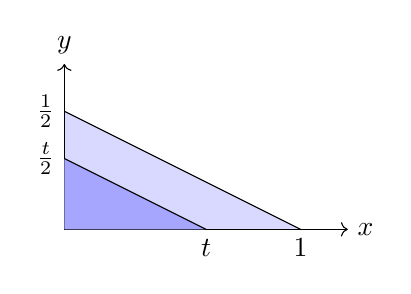
\begin{tikzpicture}[scale=3]
\fill[blue!15](0,0)--(1,0)--(0,0.5)--cycle;
\draw[->](0,0)--(1.2,0)node[right]{$x$};
\draw[->](0,0)--(0,0.7)node[above]{$y$};
\draw(0,0.5)--(1,0);
\fill[blue!35](0,0)--(0.6,0)--(0,0.3)--cycle;
\draw(0,0.3)--(0.6,0);
\node[left]at(0,0.5){$\frac12$};\node[left]at(0,0.3){$\frac t2$};
\node[below]at(1,0){$1$};\node[below]at(0.6,0){$t$};
\end{tikzpicture}
\end{center}

\section*{Problem 2}
Let $X_1,X_2,\dots\sim\operatorname{Exp}(1/5)$ be the times between customers under 30, and $Y_1,Y_2,\dots\sim\operatorname{Exp}(1/10)$ those between customers over 30. We have $\E X_i=5$, $DX_i=25$.
\begin{enumerate}
\item
\[
\P(X_1+\dots+X_{100}<480)
=\P\left(\frac{X_1+\dots+X_{100}-100\cdot5}{\sqrt{25}\sqrt{100}}
<\frac{-20}{\sqrt{25\cdot100}}\right)
\approx\Phi(-0.4)\approx\boxed{34.458\%}.
\]
\item
\[
Z_1:=\min(X_1,Y_1)\sim\operatorname{Exp}(\tfrac15+\tfrac1{10})
=\operatorname{Exp}(\tfrac3{10}).
\]
\item If $Z_i$ is the time between customers $i-1$ and $i$, then
$Z_i\sim\operatorname{Exp}(3/10)$, $\E Z_i=10/3$, $DZ_i=(10/3)^2$. Hence
\[
\P(Z_1+\dots+Z_{150}<480)
=\P\left(\frac{Z_1+\dots+Z_{150}-500}{\sqrt{150}\,(10/3)}
<\frac{-20}{\sqrt{150}\,(10/3)}\right)
\approx\Phi(-0.49)\approx31.287\%.
\]
Both approximations use the CLT.
\end{enumerate}

\section*{Problem 3}
Let $X_i,Y_i$ be the horizontal and vertical components of step $i$.
Each of $(1,0),(0,1),(-1,0),(0,-1)$ has probability $1/4$.
Thus $\E X_1=\frac14-\frac14+0\cdot\frac12=0$ and
\[
\E X_1^2=\tfrac14+\tfrac14=\tfrac12,\qquad\boxed{DX_1=\tfrac12}.
\]
\begin{enumerate}
\item
\[
\P(X_1+\dots+X_{1000}>10)
=\P\left(\frac{X_1+\dots+X_{1000}}{\sqrt{1/2}\sqrt{1000}}>
\frac{10}{\sqrt{500}}\right).
\]
The handwritten CLT approximation is written as $\Phi(0.45)\approx\boxed{32.636\%}$.
\item Write $d$ for distance after 100 steps. By symmetry,
\begin{align*}
\E d^2&=\E[(X_1+\dots+X_{100})^2+(Y_1+\dots+Y_{100})^2]\\
&=2\E[(X_1+\dots+X_{100})^2]\\
&=2\left(100\E X_1^2+2\sum_{i\neq j}\E[X_iX_j]\right)
=200\E X_1^2=\boxed{100}.
\end{align*}
The mixed expectations vanish because different steps are independent and $\E X_i=0$.
For the bonus, use $(X_i,Y_i)\indep(X_j,Y_j)$ when $i\neq j$, and $X_iY_i=0$ always:
\begin{align*}
\E[(d^2)^2]
&=2\E[(X_1+\dots+X_{100})^4]\\
&\quad+2\E[(X_1+\dots+X_{100})^2(Y_1+\dots+Y_{100})^2]\\
&=2\left(100\E X_1^4+\binom{100}{2}\binom42(\E X_1^2)^2\right)\\
&\quad+2\left(100\E[X_1^2Y_1^2]+100\cdot99(\E X_1^2)^2\right)\\
&=2\left(100\cdot\tfrac12+50\cdot99\cdot6(\tfrac12)^2\right)
+200\cdot99(\tfrac12)^2.
\end{align*}
Here $\E[X_1^2Y_1^2]=0$. Therefore
\[
D(d^2)=\E[(d^2)^2]-(\E d^2)^2=\boxed{9900}.
\]
For $n$ steps, $\E d^2=n$ and
\begin{align*}
\E[(d^2)^2]
&=2\E[(X_1+\dots+X_n)^4]
+2\E[(X_1+\dots+X_n)^2(Y_1+\dots+Y_n)^2]\\
&=2n\E X_1^4+2\frac{n(n-1)}2\,6(\E X_1^2)^2
+2n(n-1)(\E X_1^2)^2\\
&=n+\tfrac32n(n-1)+\tfrac12n(n-1)=2n^2-n.
\end{align*}
Hence $\boxed{D(d^2)=2n^2-n-n^2=n^2-n}$.
\end{enumerate}

\section*{Problem 4}
\begin{enumerate}
\item $\E X_n=2\E X_{n-1}$, so $\E X_n=2^n$.
Also $DX_n=4DX_{n-1}+1$, with $DX_0=1$.
Set $a_n=DX_n$. From $a_n=4a_{n-1}+1$ and $a_{n-1}=4a_{n-2}+1$,
\[
a_n-5a_{n-1}+4a_{n-2}=0.
\]
The characteristic equation $t^2-5t+4=0$ has roots 4 and 1, hence
$a_n=C_1\,4^n+C_2$. Since $a_0=1,a_1=5$,
\[
C_1+C_2=1,\quad4C_1+C_2=5,\quad C_1=\tfrac43,\quad C_2=-\tfrac13.
\]
Thus $\boxed{DX_n=\tfrac13(4^{n+1}-1)}$.
\item $\E(X_i-2X_{i-1})^2=\E\epsilon_i^2=1$, so $\boxed{\E S_{n,1}=n}$.
For the absolute-value term, the handwritten intermediate line is
$\E|X_n-2X_{n-1}|^2=\E|\epsilon_i|$. The notes then use
\begin{align*}
\E|N(0,1)|
&=\int_{-\infty}^\infty |x|\frac1{\sqrt{2\pi}}e^{-x^2/2}\,dx\\
&=2\int_0^\infty\frac{x}{\sqrt{2\pi}}e^{-x^2/2}\,dx
=\frac2{\sqrt{2\pi}}\int_0^\infty e^{-x^2/2}\,d(x^2/2)
=\sqrt{\frac2\pi}.
\end{align*}
Therefore $\boxed{\E S_{n,2}=n\sqrt{2/\pi}}$.
\item If $\epsilon_i\sim N(1,2)$, then $\E\epsilon_i=1$, $D\epsilon_i=2$.
We have $\E X_n=2\E X_{n-1}+1$, $\E X_0=1$. For
$a_n=2a_{n-1}+1$, $a_0=1,a_1=3$,
\[
a_n-3a_{n-1}+2a_{n-2}=0,\qquad a_n=C_1\,2^n+C_2.
\]
The equations $C_1+C_2=1$, $2C_1+C_2=3$ give
$\boxed{\E X_n=2^{n+1}-1}$.
Similarly, $DX_n=4DX_{n-1}+2$ has form $C_1\,4^n+C_2$, with
$DX_0=1,DX_1=6$, giving
\[
\boxed{DX_n=\tfrac13(5\cdot4^n-2)}.
\]
The notes calculate
\begin{align*}
\E S_{n,1}&=n\E[N(1,2)^2]=n(2^2-1)=3n,\\
\E S_{n,2}&=n\E|N(1,2)|^2=n\E|\sqrt2Z+1|,\quad Z\sim N(0,1).
\end{align*}
Writing $\varphi$ for the standard normal density,
\begin{align*}
\E|\sqrt2Z+1|
&=\int_{-\infty}^\infty|\sqrt2x+1|\varphi(x)\,dx\\
&=\int_{-\sqrt2/2}^\infty(\sqrt2x+1)\varphi(x)\,dx
-\int_{-\infty}^{-\sqrt2/2}(\sqrt2x+1)\varphi(x)\,dx\\
&=\int_{-\sqrt2/2}^\infty\varphi(x)\,dx
-\int_{-\infty}^{-\sqrt2/2}\varphi(x)\,dx\\
&\quad+\int_{-\sqrt2/2}^\infty\sqrt2x\varphi(x)\,dx
+\int_{\sqrt2/2}^\infty\sqrt2x\varphi(x)\,dx\\
&=\Phi(\tfrac{\sqrt2}{2})-(1-\Phi(\tfrac{\sqrt2}{2}))
+\frac1{\sqrt\pi}\left[
\int_{-\sqrt2/2}^{\sqrt2/2}xe^{-x^2/2}\,dx
+2\int_{\sqrt2/2}^\infty xe^{-x^2/2}\,dx\right]\\
&=2\Phi(\tfrac{\sqrt2}{2})-1+
\frac2{\sqrt\pi}e^{-1/4}\approx1.3993.
\end{align*}
The symmetric integral is zero.
\end{enumerate}
The final general formula in the handwritten source is
\[
X\sim N(\mu,\sigma^2):\qquad
\E|X|=\mu(2\Phi(\mu/\sigma)-1)
+\sigma\sqrt{\frac2\pi}e^{-\mu^2/(2\sigma^2)}.
\]
See the folded normal distribution.
\end{document}
